\documentclass[11pt, a4paper]{article}

% =====================================================================
% 1. 기본 패키지 및 한국어 설정
% =====================================================================
\usepackage[utf8]{inputenc}
\usepackage{kotex}           % 한글 지원을 위한 필수 패키지
\usepackage[margin=1in]{geometry} % 여백 설정
\usepackage{amsmath, amssymb}% 수학 공식 패키지
\usepackage{graphicx}        % 이미지 삽입 패키지
\usepackage{booktabs}        % 학술지 스타일 테이블 패키지
\usepackage{hyperref}        % 하이퍼링크 및 북마크
\usepackage{float}           % 그림/표의 정확한 위치 조절 ([H])
\usepackage{cite}            % 인용 관리 패키지
\usepackage{subcaption}      % 하위 그림 구성 패키지
\usepackage{titlesec}        % 섹션 스타일 지정 패키지
\usepackage{tcolorbox}       % 경고창/요약창 구현용 패키지

% =====================================================================
% 2. 스타일 정의 및 하이퍼링크 세부 설정
% =====================================================================
\hypersetup{
    colorlinks=true,
    linkcolor=blue,
    filecolor=magenta,      
    urlcolor=cyan,
    pdftitle={Physical Laws that Hide like a Chameleon},
    pdfauthor={Dongkyu Lee},
}

% 섹션 제목 스타일 수정
\titleformat{\section}{\large\bfseries}{\thesection.}{0.5em}{}
\titleformat{\subsection}{\normalsize\bfseries}{\thesubsection}{0.5em}{}

% =====================================================================
% 3. 표지 정보 정의
% =====================================================================
\title{
    \bfseries\Large 
    Physical Laws that Hide like a Chameleon: Environmental Density-Dependent Dynamics Simulation
}
\author{
    \textbf{이동규} \\
    \small 서울대학교 물리천문학부 물리학전공 \\
}
\date{2026년 5월 31일 (2026년 7월 10일 수정·검증), 총 소요시간: 8시간}

% =====================================================================
% 4. 본문 작성
% =====================================================================
\begin{document}

\maketitle

\begin{abstract}
본 연구에서는 카멜레온 메커니즘(Chameleon Mechanism)의 밀도 종속적 차폐를 무차원 고전 동역학 모형으로 구현하였다. 정적 스칼라 장은 1차원 전이 밀도와 구형 대칭 밀도에서 경계값 문제(BVP)로 풀고, 시험 입자의 궤도는 적응형 Dormand--Prince RK45 초기값 문제(IVP)로 적분하였다. 수치 방법의 재현성을 위해 허용오차, 경계조건, 무차원화 계수를 명시하고, 직접 구현한 고정 간격 RK4와 비교하였다. 코드는 해석적 조화진동자, 균일밀도의 상수 장 해, 에너지 보존으로 검증되었으며 RK4 관측 수렴차수는 4.004, 전체 모형의 RK4--RK45 최대 상태 차이는 $5.0\times10^{-11}$이었다. 가우시안 무작위 밀도장의 복잡한 위상 궤적에는 에너지 오차, 귀환주기, 유한시간 Lyapunov 지수를 추가하였다. 그 결과 이 계는 비선형적으로 변형되지만 시간에 무관한 1차원 보존계이므로 결정론적 카오스의 증거가 없음을 확인하였다. 마지막으로 진공 챔버에서 원자 센서와 벌크 센서가 동일한 장 구배에 서로 다른 스칼라 전하로 반응하는 검출 원리를 제시하고, 본 무차원 계산이 특정 $(M,n,\beta)$의 실험적 허용성을 직접 주장하지 않는다는 한계를 명확히 하였다.
\end{abstract}

% ---------------------------------------------------------------------
% 1. 서론
% ---------------------------------------------------------------------
\section{서론 (Introduction)}

\subsection{우주론적 배경 및 문제 제기}
현대 우주론에서 암흑 에너지(Dark Energy)의 실체를 설명하는 것은 주요 과제 중 하나이다. 아인슈타인의 우주 상수($\Lambda$) 모델은 미세 조정 문제(Fine-tuning problem)와 우주론적 일치성 문제(Coincidence problem)를 내포하고 있어, 시간에 따라 진화하는 스칼라 필드($\phi$)를 도입하는 대안 중력 및 퀸테센스(Quintessence) 이론들이 제시되어 왔다.

일반적으로 스칼라 필드가 존재하고 일반 물질(Standard Model matter)과 결합한다면, 이는 물질 사이의 상호작용을 매개하는 제5의 힘(Fifth Force)을 유도하게 된다. 그러나 지구 상의 정밀 비틀림 저울 실험이나 태양계 내 천체들의 궤도 관측(예: 달 레이저 거리 측정 시험 등)을 통해 일반 상대성 이론(General Relativity)의 등가원리가 고도의 정밀도로 성립함이 확인되었으며, 제5의 힘은 검출되지 않았다. 우주론적 스케일의 스칼라 필드 작용 요건과 국소적 실험의 미검출 사실 간의 상충 관계는 이론 물리학의 주요 난제였다.

\subsection{카멜레온 메커니즘의 이론적 출발점}
이 모순을 타개하기 위해 2004년 저스틴 쿠리(Justin Khoury)와 아만다 웰트먼(Amanda Weltman)은 카멜레온 스크리닝 효과(Chameleon Screening Effect)를 제안하였다\cite{Khoury2004prl, Khoury2004prd}. 이 이론의 주요 가정은 물리 법칙이나 작용 상수가 온 우주에서 균일하게 불변하는 것이 아니라, 주변 환경의 물질 밀도(Density)에 반응하여 동적으로 조절된다는 점이다.

카멜레온 장의 거동 방식은 다음과 같이 요약된다.
\begin{itemize}
    \item \textbf{고밀도 환경 (예: 지구 표면, 실험실 용기 벽, 항성 내부):} 장의 유효 질량이 무거워진다. 힘의 전달 범위인 컴프턴 파장($\lambda_c \sim 1/m_{\text{eff}}$)이 수 마이크로미터 혹은 그 이하의 스케일로 수축하여 장의 분포가 차단(Screening)되며, 제5의 힘은 관측 한계 이하로 억제된다.
    \item \textbf{저밀도 환경 (예: 은하 간 진공 공간인 Cosmic Void):} 장의 유효 질량이 극도로 가벼워져 컴프턴 파장이 거대 스케일로 확장된다. 이에 따라 제5의 힘의 작용 범위가 복원되어 우주 가속 팽창과 거대 구조 형성에 기여하게 된다.
\end{itemize}

\subsection{본 텀 프로젝트의 목적 및 범위}
본 연구는 공간상에 밀도 구배(Density Gradient)가 존재할 때 일어나는 물리적 법칙의 전이 현상을 역학계 수치 시뮬레이션을 통해 직접 실증하는 것을 목적으로 한다.

이를 위해 공간상에서 밀도가 연속적으로 변화하는 가상의 1차원 역학계 및 2차원 구형 대칭 천체 모델을 설정하고, 이곳을 통과하는 시험 입자(Test Particle)의 복합 운동 궤적을 연산한다. 고밀도 차폐 영역에서 저밀도 비차폐 영역으로 입자가 진입하고 탈출할 때 겪는 물리적 힘의 동역학적 전이를 위상 공간(Phase Space, $x-v$) 상의 궤적으로 나타내어, 카멜레온 장의 반응 속성을 정량적으로 분석한다. 더 나아가 공간 밀도가 불규칙하게 요동치는 현실적인 우주 무작위 매질에서의 운동 시나리오를 설계하여 동역학계 모델을 확장한다.

모든 소스 코드, 실행 방법, 검증 지표 JSON은 공개 저장소
\href{https://github.com/Lasqui-Ponto/Mechanics_Term_Project}{github.com/Lasqui-Ponto/Mechanics\_Term\_Project}에서 확인할 수 있다.

% ---------------------------------------------------------------------
% 2. 물리학적 배경 이론
% ---------------------------------------------------------------------
\section{물리학적 배경 이론 (Physical Background Theory)}

\subsection{유효 포텐셜과 밀도 종속 유효 질량 (Effective Potential \& Effective Mass)}
카멜레온 스칼라 필드 $\phi$가 자체적인 런어웨이 포텐셜 $V(\phi)$를 갖고, 물질 장(Matter field)과 결합(Conformal Coupling)을 이루는 경우, 물질 밀도 $\rho_m$이 존재하는 환경에서의 행동 양식은 유효 포텐셜(Effective Potential, $V_{\text{eff}}$)로 기술된다.

\begin{equation}
    V_{\text{eff}}(\phi) = V(\phi) + \rho_m e^{\beta \phi / M_{\text{Pl}}}
\end{equation}

여기서 물리 변수 및 상수는 다음과 같다.
\begin{itemize}
    \item $\rho_m$: 주변 물질의 국소 질량 밀도 (Local Matter Density)
    \item $\beta$: 스칼라 필드와 일반 물질 사이의 무차원 결합 상수 (Coupling Constant)
    \item $M_{\text{Pl}}$: 축소 플랑크 질량 (Reduced Planck Mass, $\approx 2.43 \times 10^{18} \text{ GeV}$)
\end{itemize}

스칼라 필드의 자체 포텐셜 $V(\phi)$는 일반적으로 라트라-피블스(Ratra-Peebles) 모델을 따른다.

\begin{equation}
    V(\phi) = \frac{M^{4+n}}{\phi^n} \quad (n > 0)
\end{equation}

여기서 $M$은 특정 에너지 스케일이다. 필드의 값 $\phi$가 0에 가까워질 때($\phi \to 0$), 자체 포텐셜 $V(\phi)$는 무한대로 발산한다. 반대로 $\phi$가 커질수록 결합 항인 $\rho_m e^{\beta \phi / M_{\text{Pl}}}$이 지배하여 지수함수적으로 증가한다.

자체 포텐셜과 결합 항의 상호 작용으로 인해 유효 포텐셜은 유일한 평형 극솟값 $\phi_{\text{min}}$을 가지며, 이는 1차 도함수가 0이 되는 지점으로 결정된다.

\begin{equation}
    V'_{\text{eff}}(\phi_{\text{min}}) = -n \frac{M^{4+n}}{\phi_{\text{min}}^{n+1}} + \frac{\beta \rho_m}{M_{\text{Pl}}} e^{\beta \phi_{\text{min}} / M_{\text{Pl}}} = 0
\end{equation}

$\beta \phi_{\text{min}} / M_{\text{Pl}} \ll 1$ 조건 하에서 지수함수를 선형 근사($e^x \approx 1+x$)하여 전개하면, 카멜레온 장의 평형 상태 값 $\phi_{\text{min}}$은 주변 밀도에 반비례하는 형태로 결정된다.

\begin{equation}
    \phi_{\text{min}}(\rho_m) \approx \left( \frac{n M^{4+n} M_{\text{Pl}}}{\beta \rho_m} \right)^{\frac{1}{n+1}}
\end{equation}

이 평형 위치 $\phi_{\text{min}}$에서 장의 곡률(Curvature)을 구하면, 카멜레온 장의 유효 질량 $m_{\text{eff}}$를 도출할 수 있다.

\begin{equation}
    m_{\text{eff}}^2(\rho_m) = \left. \frac{d^2 V_{\text{eff}}}{d\phi^2} \right|_{\phi_{\text{min}}} = V''(\phi_{\text{min}}) + \frac{\beta^2 \rho_m}{M_{\text{Pl}}^2} e^{\beta \phi_{\text{min}} / M_{\text{Pl}}}
\end{equation}

평형 조건을 결합하여 정리하면 유효 질량과 밀도 간의 비선형적 비례 관계를 얻는다.

\begin{equation}
    m_{\text{eff}}^2(\rho_m) \approx n(n+1)\frac{M^{4+n}}{\phi_{\text{min}}^{n+2}} \propto \rho_m^{\frac{n+2}{n+1}}
\end{equation}

\begin{tcolorbox}[colback=blue!5!white,colframe=blue!75!black,title=\textbf{유효 질량의 밀도 종속성과 차폐 현상}]
\begin{itemize}
    \item \textbf{고밀도 환경 (매우 큰 $\rho_m$):}
    $\phi_{\text{min}}$이 매우 작아지며, 이에 따라 유효 질량 $m_{\text{eff}}$가 크게 증가한다. 힘의 도달 범위인 컴프턴 파장 $\lambda_c \sim 1/m_{\text{eff}}$는 마이크로미터 이하 수준으로 수축하여 차폐(screened)되며, 제5의 힘은 억제된다.
    \item \textbf{저밀도 환경 (매우 작은 $\rho_m$):}
    $\phi_{\text{min}}$이 커짐에 따라 유효 질량 $m_{\text{eff}}$가 0에 가깝게 감소한다. 컴프턴 파장 $\lambda_c$가 거대 스케일로 확장되어 비차폐(unscreened) 상태가 되고 제5의 힘이 전달된다.
\end{itemize}
\end{tcolorbox}

\subsection{얇은 껍질 효과 (Thin-Shell Screening Effect)}
반지름 $R_c$, 내부 균일 밀도 $\rho_c$를 갖는 구형 천체가 외부 진공 밀도 $\rho_0$ 환경에 놓여 있는 계를 가정한다. 천체의 질량이 크더라도 외부 시험 입자에 작용하는 카멜레온 제5의 힘이 특정 두께의 표면층에 의해서만 생성되는 현상을 얇은 껍질 효과(Thin-Shell Effect)라고 한다.

천체 내부 깊은 곳($r \ll R_c$)에서는 밀도 $\rho_c$가 매우 높기 때문에 장이 평형 상태 $\phi_c$에 결박된다. 내부 전체 공간에서 장이 상수를 유지하여 기울기가 0이 되므로 ($\nabla \phi \approx 0$), 천체 내부 질량의 대부분은 외부로 전파되는 카멜레온 장의 형성(Flux)에 기여하지 않는다.

오직 천체의 최외곽 표면 부근의 얇은 두께 $\Delta R_c$ 영역(Thin-Shell)에 존재하는 물질만이 외부 진공 값 $\phi_0$로 전이하는 기울기를 가지며 외부 장을 형성한다. 이 얇은 외피 껍질의 비율은 다음과 같이 나타난다.

\begin{equation}
    \frac{\Delta R_c}{R_c} \approx \frac{\phi_0 - \phi_c}{6 \beta M_{\text{Pl}} \Phi_N} \ll 1
\end{equation}

여기서 $\Phi_N = \frac{G M_{\text{body}}}{R_c}$는 천체의 표면 뉴턴 중력 퍼텐셜이다. 이로 인해 외부 공간의 시험 입자가 겪는 카멜레온 제5의 힘 $F_5$는 뉴턴 중력 $F_{\text{Gravity}}$에 비해 다음과 같이 억제된다.

\begin{equation}
    F_5 \approx 2 \beta^2 \left( 3\frac{\Delta R_c}{R_c} \right) F_{\text{Gravity}} \ll F_{\text{Gravity}}
\end{equation}

이러한 메커니즘을 통해 지구 및 태양과 같은 거대 천체들은 등가원리 검증 실험의 오차 범위 내에서 일반 상대론의 예측치 및 뉴턴 역학적 거동과 일치하는 결과를 유지할 수 있다.

% ---------------------------------------------------------------------
% 3. 선행 연구 조사
% ---------------------------------------------------------------------
\section{선행 연구 조사 (Literature Review)}

본 텀 프로젝트의 기초가 되는 두 선행 연구의 주요 기여는 다음과 같이 정리할 수 있다.

\subsection{Khoury \& Weltman (2004) - PRL 논문}
\begin{itemize}
    \item \textbf{논문 정보:} Justin Khoury and Amanda Weltman, ``Chameleon Fields: Awaiting Surprises for Tests of Gravity in Space,'' \textit{Physical Review Letters}, Vol. 93, Art. No. 171104 (2004)\cite{Khoury2004prl}.
    \item \textbf{주요 내용 및 기여:} 
    카멜레온 메커니즘을 최초로 제시한 연구이다. 등가원리의 정밀한 성립 범위 내에서 우주론적 스칼라 필드가 공존할 수 있음을 수학적으로 논증하였다.
    지상 실험실 환경의 진공 챔버 용기 벽면이 카멜레온 장의 입장에서는 고밀도 장벽으로 작용하여 필드가 차폐됨을 규명하였다. 반면 대기 밀도가 거의 없는 우주 공간(Space)에서는 이러한 차폐 효과가 감쇄되어 제5의 힘이 전달될 수 있음을 지적하여, 향후 위성을 통한 등가원리 위배 실험의 이론적 토대를 마련하였다.
\end{itemize}

\subsection{Khoury \& Weltman (2004) - PRD 논문}
\begin{itemize}
    \item \textbf{논문 정보:} Justin Khoury and Amanda Weltman, ``Chameleon Cosmology,'' \textit{Physical Review D}, Vol. 69, Art. No. 044026 (2004)\cite{Khoury2004prd}.
    \item \textbf{주요 내용 및 기여:}
    PRL 논문이 실험실 규모의 검증 가능성에 초점을 맞춘 반면, 본 PRD 논문은 우주론적 시나리오와 장 이론적 전개를 구체화하였다.
    다양한 물질 상태 방정식(Equation of State) 하에서 카멜레온 필드의 진화 방식을 분석하였으며, 결합 계수 $\beta$가 존재하는 환경에서도 우주 마이크로파 배경(CMB) 온도 요동 복사 이방성 및 거대 구조 형성(LSS) 관측 한계와 정합성을 이루는 매개변수 허용 영역(Parameter space)을 수식 전개를 통해 도출하였다.
\end{itemize}

% ---------------------------------------------------------------------
% 4. 시뮬레이션 물리 모델링 및 지배 방정식
% ---------------------------------------------------------------------
\section{시뮬레이션 물리 모델링 및 지배 방정식 (Dynamics Simulation)}

\subsection{무차원화와 해석 범위}
물리 변수에 $x=L_0\hat{x}$, $\phi=\Phi_0\hat{\phi}$, $\rho=\rho_0\hat{\rho}$, $t=T_0\hat{t}$를 대입하면 장 방정식과 입자 방정식의 계수는
\begin{equation}
 A=\frac{nM^{4+n}L_0^2}{\Phi_0^{n+2}},\qquad
 B=\frac{\beta\rho_0L_0^2}{M_{\mathrm{Pl}}\Phi_0},\qquad
 C=\frac{\beta\Phi_0T_0^2}{M_{\mathrm{Pl}}L_0^2}
\end{equation}
로 정리된다. 본 계산은 $n=1$에서 $A=B=C=1$로 둔 무차원 교육용 모형이다. 따라서 코드의 \texttt{BETA=1}은 정규화된 힘 계수이며, 실제 결합상수 $\beta=1$인 특정 천체물리학 모형이 관측 제약을 만족한다는 뜻이 아니다. 물리적 예측에는 $(M,n,\beta)$와 $L_0,\Phi_0,\rho_0,T_0$를 함께 지정해야 한다.

무차원 장 방정식과 국소 유효 질량 및 컴프턴 길이는
\begin{equation}
 \frac{d^2\hat{\phi}}{d\hat{x}^2}=-\frac{1}{\hat{\phi}^2}+\hat{\rho}(\hat{x})e^{\hat{\phi}},\qquad
 \hat{m}_{\mathrm{eff}}^2=\frac{2}{\hat{\phi}_{\min}^3}+\hat{\rho}e^{\hat{\phi}_{\min}},\qquad
 \hat{\lambda}_c=\hat{m}_{\mathrm{eff}}^{-1}
\end{equation}
이다. 물리 단위에서는 $\lambda_c=\hbar/(m_{\mathrm{eff}}c)$이며 자연단위에서는 $1/m_{\mathrm{eff}}$이다. 본 모형의 균일 극솟값은 고밀도 $\hat{\rho}=10$에서 $\hat{\phi}_{\min}=0.27553$, 저밀도 $\hat{\rho}=0.01$에서 $2.65345$이다.

\subsection{밀도 구배와 정적 장 BVP}
계산 경계는 $\hat{x}\in[-20,20]$로 넓게 잡고 결과는 $[-12,12]$에서 표시하였다. 이렇게 하면 입자 궤도가 장 해의 경계에 접근하지 않고, 경계층이 관심 영역에 섞이는 것을 방지할 수 있다. 밀도는
\begin{equation}
 \hat{\rho}(\hat{x})=\frac{\hat{\rho}_{\mathrm{high}}+\hat{\rho}_{\mathrm{low}}}{2}
 -\frac{\hat{\rho}_{\mathrm{high}}-\hat{\rho}_{\mathrm{low}}}{2}
 \tanh\!\left(\frac{\hat{x}}{\hat{w}}\right)
\end{equation}
으로 두었으며 $(\hat{\rho}_{\mathrm{high}},\hat{\rho}_{\mathrm{low}},\hat{w})=(10,0.01,1.5)$이다. 경계조건은
\begin{equation}
 \hat{\phi}(-20)=\hat{\phi}_{\min}(10),\qquad
 \hat{\phi}(20)=\hat{\phi}_{\min}(0.01)
\end{equation}
이다. \texttt{scipy.integrate.solve\_bvp}의 4차 collocation과 적응 격자를 사용하였고, 잔차 허용오차는 $10^{-6}$, 최대 노드 수는 30,000으로 설정하였다. 해가 수렴하지 않으면 코드는 결과를 저장하지 않고 예외를 발생시킨다.

\subsection{입자 IVP와 RK45 적응 적분}
시험 입자 자체의 차폐를 $Q_{\mathrm{test}}\in[0,1]$인 스칼라 전하로 쓰면
\begin{equation}
 \frac{d^2\hat{x}}{d\hat{t}^2}=-\hat{k}\hat{x}
 -Q_{\mathrm{test}}\frac{d\hat{\phi}}{d\hat{x}},\qquad \hat{k}=0.15
\end{equation}
이다. 궤도 시각화에서는 비차폐 시험 입자 $Q_{\mathrm{test}}=1$을 사용하였다. 초기조건은 $(\hat{x}_0,\hat{v}_0)=(-8,2)$이고, 입자는 계산 경계에서 충분히 떨어진 상태를 유지한다.

IVP는 Dormand--Prince 5(4) 쌍인 \texttt{solve\_ivp(method='RK45')}로 적분하였다. 한 단계에서 5차 해를 진행값으로 쓰고 4차 내장해와의 차이로 국소 오차를 추정하여, 오차가 허용범위보다 크면 그 단계를 거부하고 간격을 줄인다. 설정값은 \texttt{rtol=$10^{-9}$}, \texttt{atol=$10^{-11}$}, \texttt{max\_step=0.05}이다.

라이브러리 결과에만 의존하지 않기 위해 고전적 고정 간격 RK4도 직접 구현하였다.
\begin{align}
 k_1&=f(t_n,y_n),& k_2&=f(t_n+h/2,y_n+hk_1/2),\\
 k_3&=f(t_n+h/2,y_n+hk_2/2),& k_4&=f(t_n+h,y_n+hk_3),\\
 y_{n+1}&=y_n+\frac{h}{6}(k_1+2k_2+2k_3+k_4).&&
\end{align}

\subsection{코드 검증과 수렴성}
검증 결과는 그림~\ref{fig:verification}과 같다. 첫째, 제5의 힘을 끈 조화진동자의 해석해
\begin{equation}
 x(t)=x_0\cos(\omega t)+\frac{v_0}{\omega}\sin(\omega t),\qquad \omega=\sqrt{k}
\end{equation}
와 RK45를 비교하였다. 둘째, 균일 밀도에서는 $\phi(x)=\phi_{\min}(\rho)$가 BVP의 정확한 상수해이므로 수치해와 비교하였다. 셋째, $h=0.4,0.2,0.1,0.05$에서 직접 RK4의 전역오차 기울기를 계산하고, 전체 카멜레온 궤도에서 RK4와 RK45 및 보존에너지
\begin{equation}
 E=\frac{1}{2}\hat{v}^2+\frac{1}{2}\hat{k}\hat{x}^2+\hat{\phi}(\hat{x})
\end{equation}
를 교차검증하였다.

\begin{figure}[H]
 \centering
 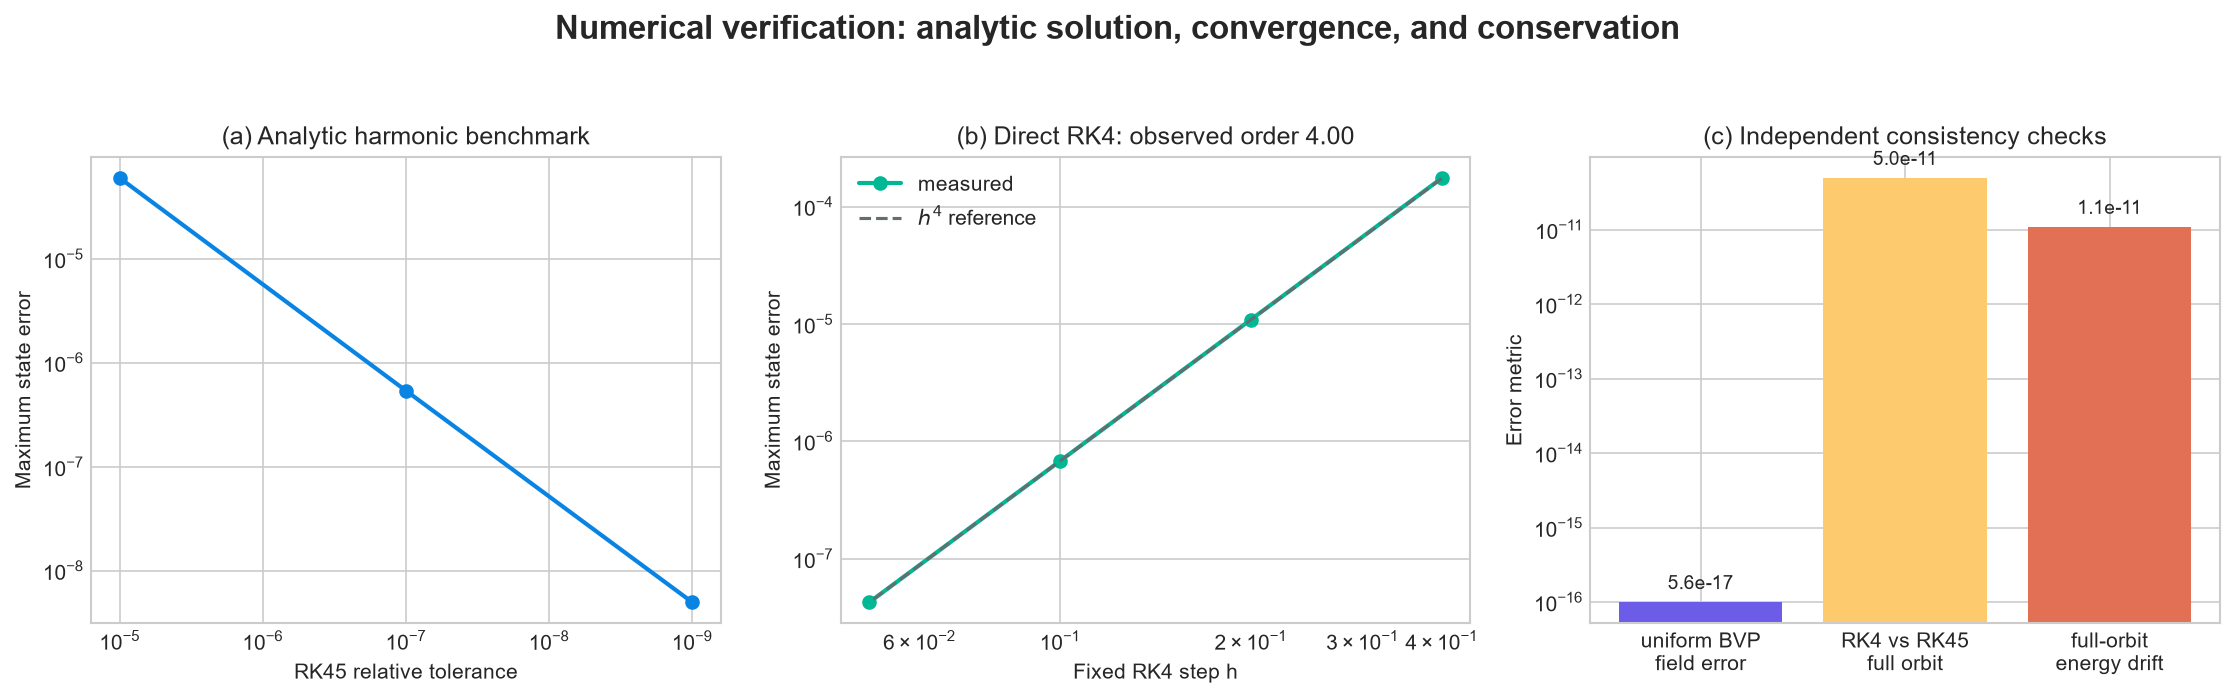
\includegraphics[width=0.98\textwidth]{verification_results.png}
 \caption{수치 코드 검증. (a) RK45 허용오차에 따른 해석적 조화진동자 최대 상태오차, (b) 직접 구현한 RK4의 $h^4$ 수렴과 관측 차수 4.004, (c) 균일밀도 BVP 오차 $5.6\times10^{-17}$, 전체 모형 RK4--RK45 최대 상태 차이 $5.0\times10^{-11}$, 최대 상대 에너지 드리프트 $1.1\times10^{-11}$.}
 \label{fig:verification}
\end{figure}

% ---------------------------------------------------------------------
% 5. 시뮬레이션 수치 해석 결과 및 고전 역학적 분석
% ---------------------------------------------------------------------
\section{시뮬레이션 수치 해석 결과 및 고전 역학적 분석 (Simulation Results)}

수치 해석을 통해 도출한 결과 및 동역학적 분석은 다음과 같다.

\subsection{1차원 입자 궤적 및 동역학 분석 대시보드 시각화 결과}
1차원 tanh 밀도 구배 환경에서의 입자 거동 대시보드는 그림~\ref{fig:dashboard}과 같다.

\begin{figure}[H]
    \centering
    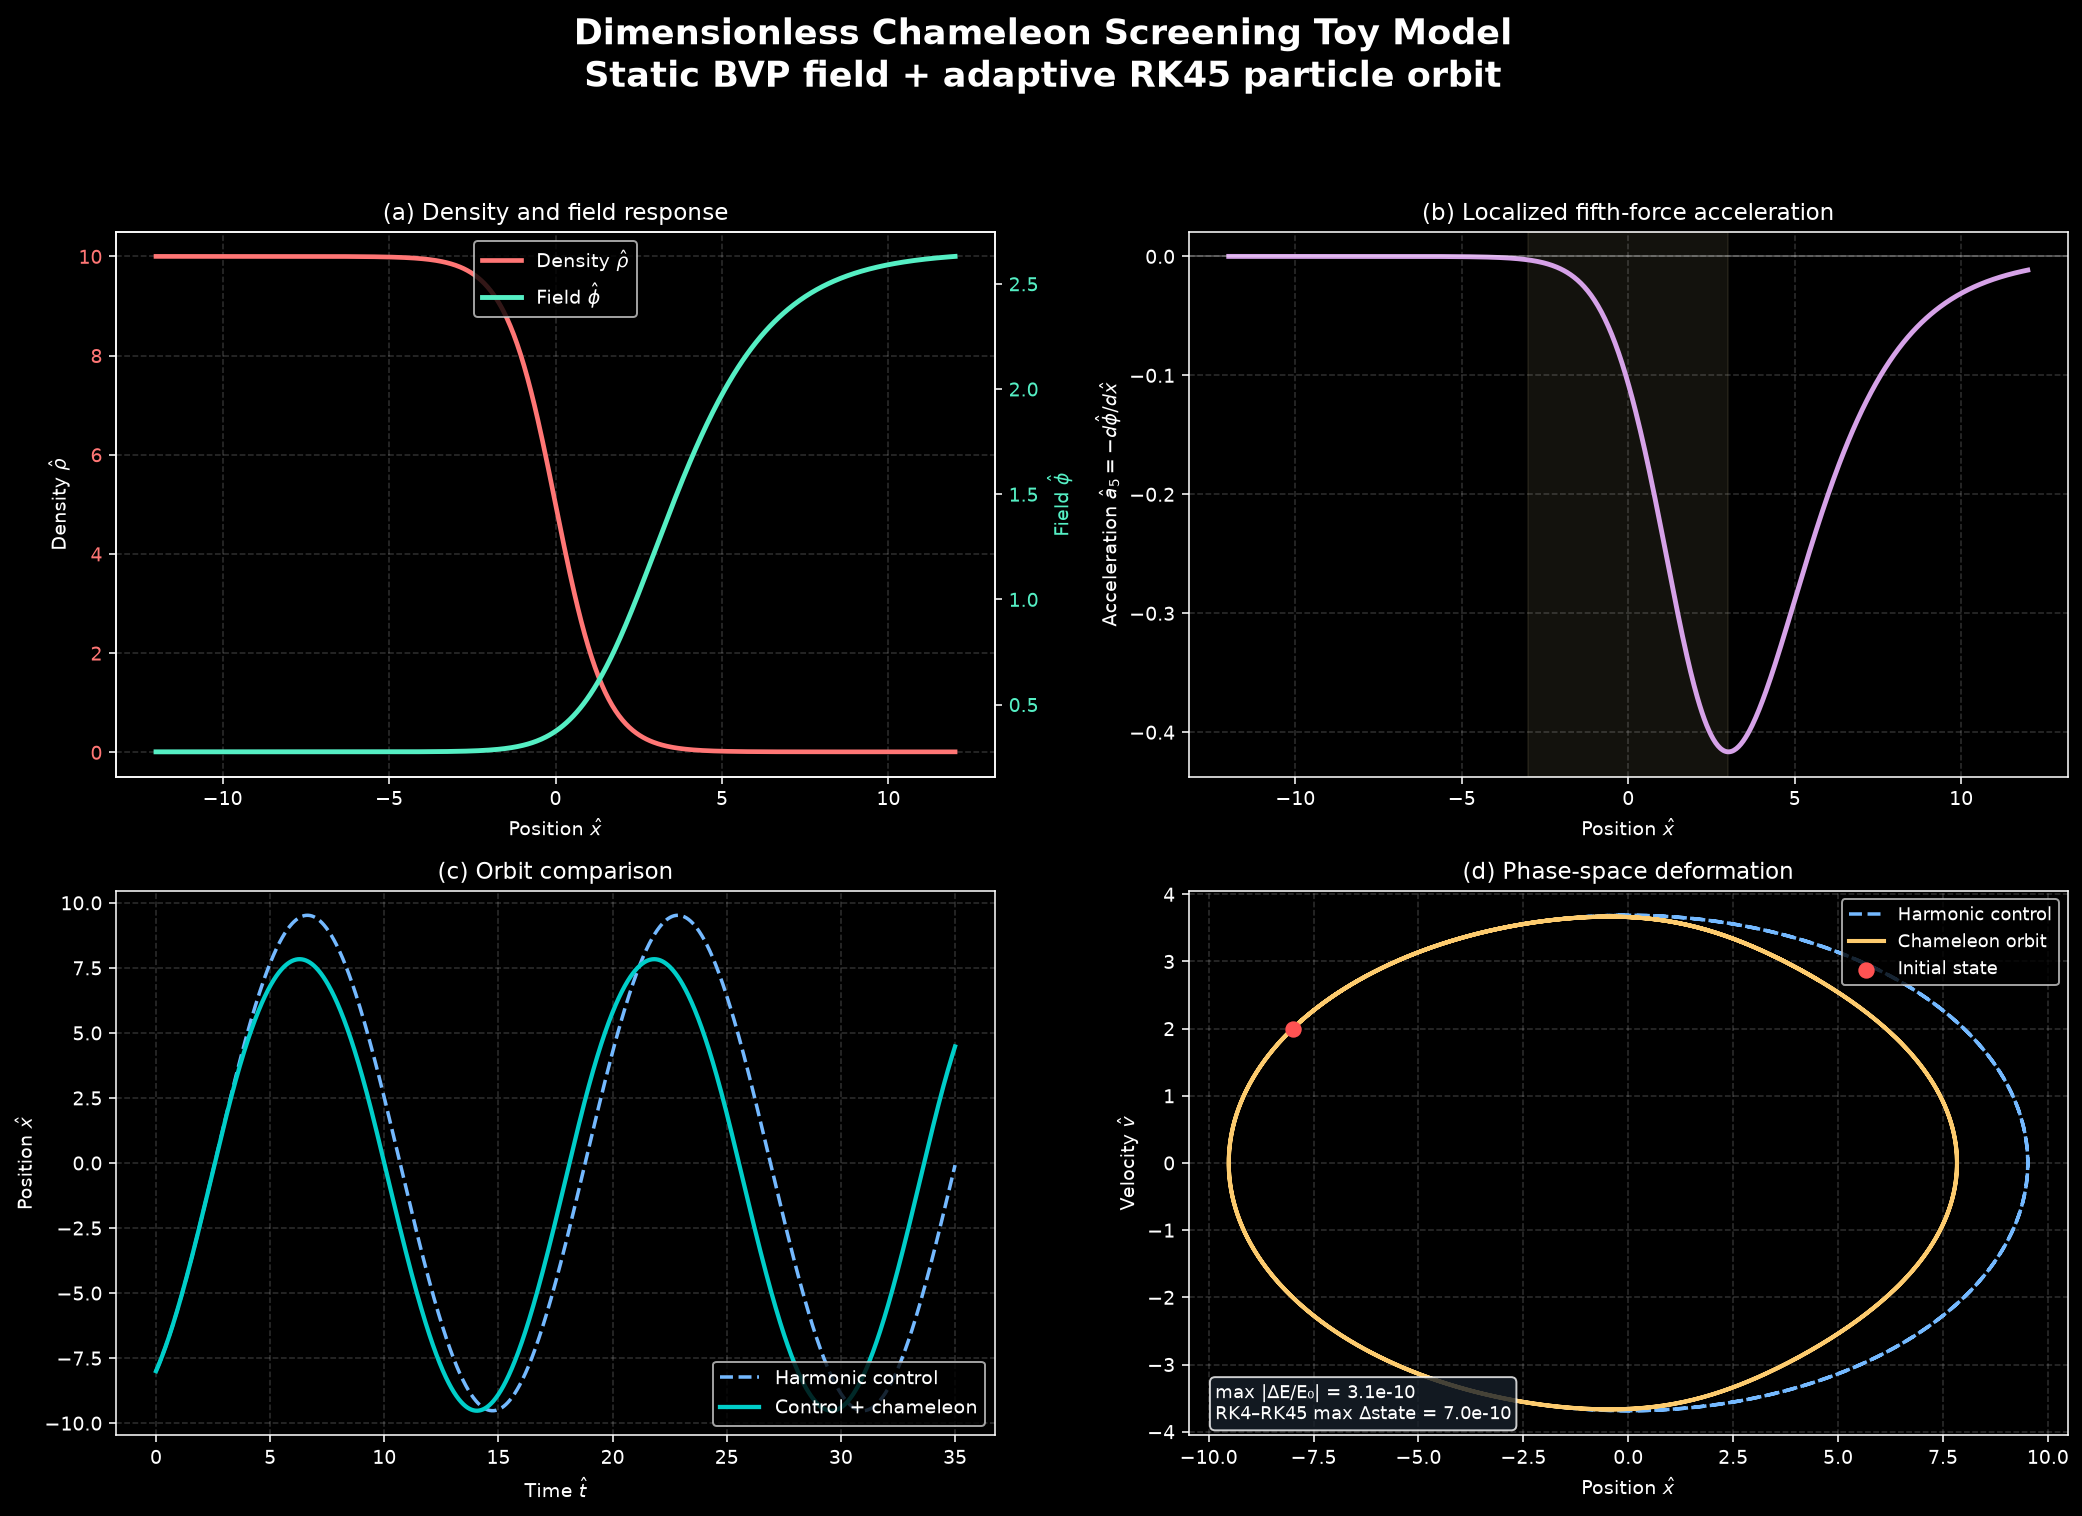
\includegraphics[width=0.9\textwidth]{chameleon_simulation_results.png}
    \caption{카멜레온 1차원 무차원 시뮬레이션 결과. (a) 밀도 $\hat\rho(\hat x)$와 장 $\hat\phi(\hat x)$, (b) $\hat a_5=-d\hat\phi/d\hat x$, (c) 조화 대조군과 카멜레온 결합군의 궤도, (d) 보존에너지 등고선에 해당하는 위상 공간 궤적. 패널 (d)에 에너지 오차와 RK4--RK45 교차검증 오차를 함께 표시하였다.}
    \label{fig:dashboard}
\end{figure}

\subsection{2D 구형 대칭 카멜레온 장 공간 분포 및 얇은 껍질 실증 결과}
구형 대칭 천체 모델에서의 카멜레온 장 수치 해석 결과는 그림~\ref{fig:spherical}과 같다.

\begin{figure}[H]
    \centering
    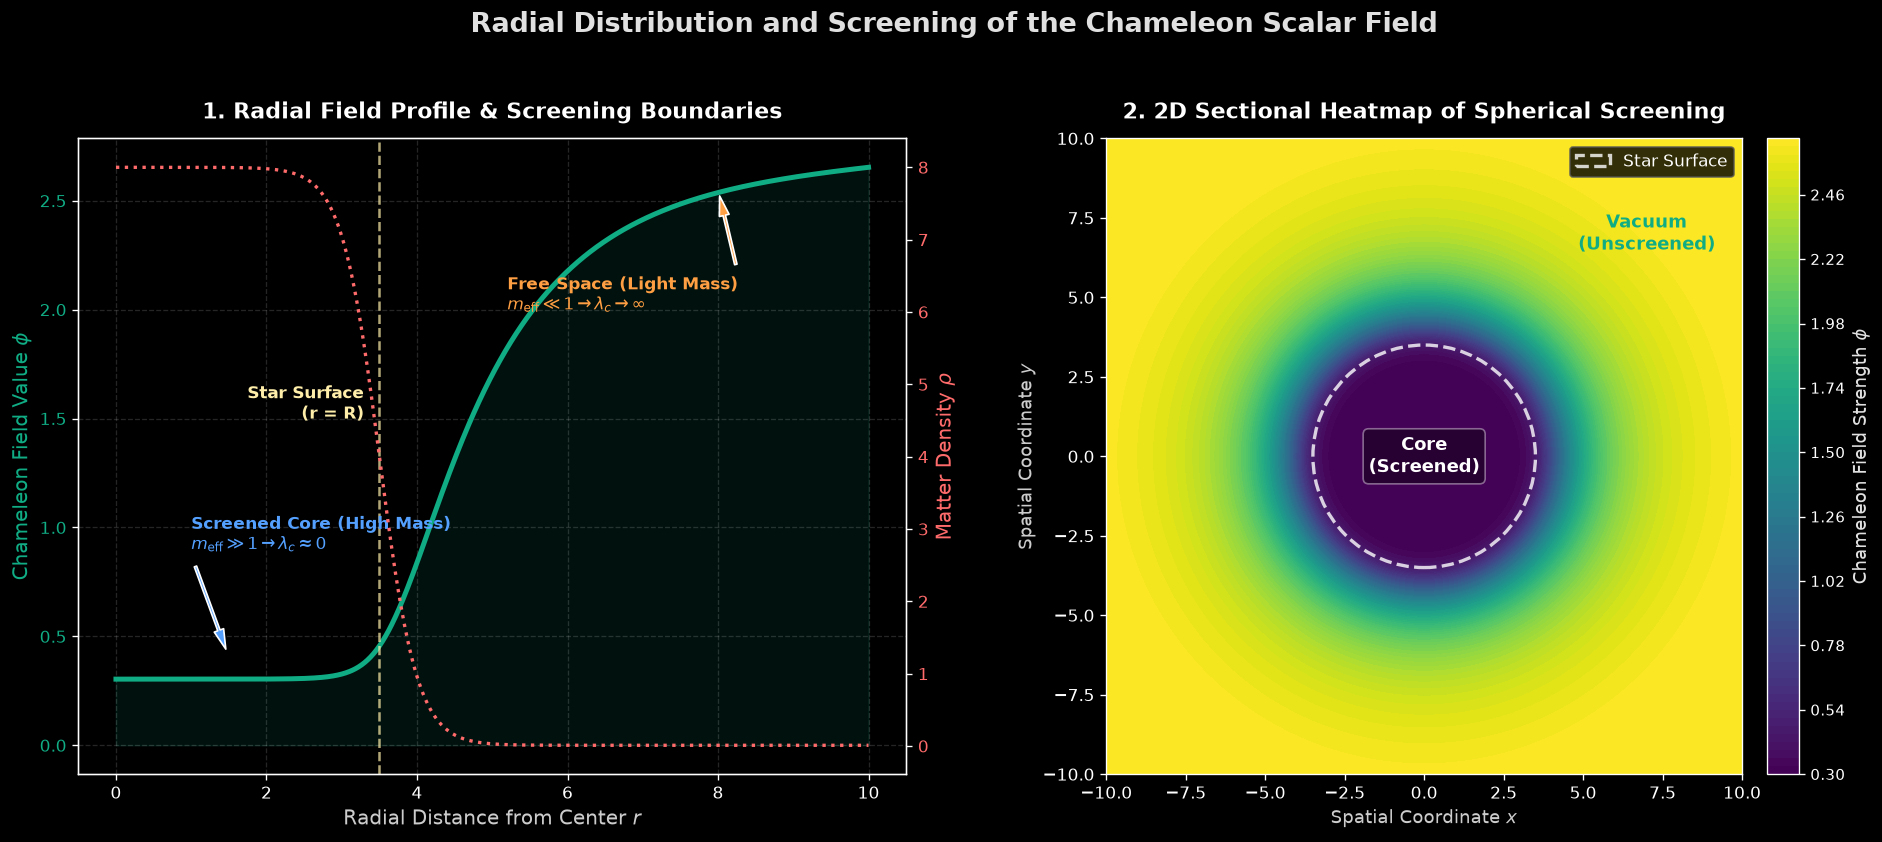
\includegraphics[width=0.9\textwidth]{chameleon_field_distribution.png}
    \caption{구형 대칭 고밀도 천체 표면에서의 카멜레온 장 분포 분석. (좌측) 1차원 Radial 축 방향 카멜레온 필드 세기 $\phi(r)$ 완화 분포 그래프, (우측) 천체 단면에 투영한 카멜레온 스크리닝 시각화 2D 단면 차폐 히트맵 (흰색 점선은 천체의 물리 표면 경계 $R=3.5$를 지정함).}
    \label{fig:spherical}
\end{figure}

\subsubsection{1D Radial Profile 분석}
그림~\ref{fig:spherical}의 좌측 그래프에서 천체 중심($r=0$)부터 표면 경계인 $r = 3.5$까지 내부 영역에서는 스칼라 필드 $\phi$의 값이 고밀도 평형값인 $\phi_{\text{body}} \approx 0.29$ 근처에 강하게 고정되어 평탄하게 유지된다. 
반면 표면을 벗어나 밀도가 낮은 진공 영역($r > 3.5$, $\rho_{\text{vacuum}} = 0.01$)으로 진출하면서 필드 강도가 급격히 상승하여 외부 진공 영역의 기댓값 $\phi_{\text{vacuum}} \approx 2.65$로 수렴한다. 이는 고밀도 영역에서 차폐된 장이 저밀도 영역으로 진입하면서 활성화되는 물리적 전이를 보여준다.

\subsubsection{2D Sectional Heatmap 분석}
그림~\ref{fig:spherical}의 우측 히트맵은 천체 내부($R < 3.5$, 흰색 점선 안쪽)에서 장의 강도가 억제(보라색)되어 차폐 상태에 머물러 있음을 보여준다.
반면 천체 표면 경계 부근에서 외부 방향으로 장의 구배가 생성되는 얇은 껍질 효과(Thin-Shell Effect)가 2차원 공간 상의 컬러 대비를 통해 확인된다. 천체의 질량이 크더라도 중심부의 질량은 장의 형성에 기여하지 않고, 오직 표면의 얇은 껍질층에 분포한 질량만이 외부 필드를 형성한다는 이론적 성질과 부합한다.

\subsection{장의 공간 분포 및 차폐 효과 (대시보드 Plot a 분석)}
그림~\ref{fig:dashboard}(a)에서 수치적으로 도출된 장의 값은 고밀도 영역의 $\phi_{\text{min}} \approx 0.276$에서 저밀도 영역의 $\phi_{\text{min}} \approx 2.653$으로 천이한다.
특히 $x < -4$ 구간에서는 밀도의 영향으로 인해 $\nabla \phi \approx 0$으로 차폐 상태를 유지하다가, 천이 영역을 벗어남에 따라 평형값이 상승하는 1차원적 위상 거동을 나타낸다.

\subsection{제5의 힘의 공간적 국소화 (대시보드 Plot b 분석)}
그림~\ref{fig:dashboard}(b)에서 제5의 힘 $F_5(x) = -\beta \frac{d\phi}{dx}$는 좌측 고밀도 영역 및 우측 저밀도 평탄 영역에서 모두 0에 수렴한다.
오직 밀도 구배가 존재하는 중앙의 전이 영역($x \in [-3, 3]$) 부근에서만 제5의 힘이 음의 방향으로 피크(Peak)를 형성하며 국소적으로 작용한다. 이는 주변 환경의 밀도 변화가 급격히 발생하는 경계에서만 숨겨져 있던 제5의 힘이 유도되고, 평탄한 공간에서는 장이 억제된다는 물리적 가시성을 실증한다.

\subsection{궤적 및 위상 공간 분석 (대시보드 Plot c \& d 분석)}
초기 조건 $\hat{x}_0=-8.0$, $\hat{v}_0=2.0$에서 출발한 시험 입자의 동역학적 분석 결과는 다음과 같다.
\begin{itemize}
    \item \textbf{시간 궤적 분석 [그림~\ref{fig:dashboard}(c)]:}
    뉴턴 중력만 작용하는 경우(Newton Only, 청색 점선) 입자는 에너지 보존에 의해 사인파 형태의 조화 운동을 반복한다. 
    반면 카멜레온 힘이 결합한 경우 고밀도 영역 내부에서는 뉴턴 궤적과 거의 일치하다가, $\hat\phi$가 증가하는 경계를 지날 때 음의 방향의 $-d\hat\phi/d\hat x$를 받아 양의 turning point가 대조군보다 작아진다. 힘의 방향은 장 구배가 결정하므로 이를 일반적인 ``척력 증폭''으로 해석해서는 안 된다.
    \item \textbf{위상 공간 ($x-v$) 분석 [그림~\ref{fig:dashboard}(d)]:}
    고전 뉴턴 보존계는 위상 평면 상에서 대칭 타원형 궤도(청색 점선)를 유지한다. 
    카멜레온 결합 궤적은 타원에서 벗어나 비대칭이지만 하나의 매끄러운 폐곡선을 이룬다. 이는 시간에 무관한 유효 퍼텐셜 $U(\hat x)=\hat k\hat x^2/2+\hat\phi(\hat x)$의 같은 에너지 등고선이며, 복잡한 모양 자체는 카오스의 증거가 아니다.
\end{itemize}

% ---------------------------------------------------------------------
% 6. 심화 연구: 불규칙한 정적 매질의 비선형 동역학
% ---------------------------------------------------------------------
\section{심화 연구: 정적 무작위 매질의 비선형 동역학과 카오스 판정}

가우시안 평활화를 거친 재현 가능한 무작위 밀도장을 난수 시드 137로 생성하였다. 계산 경계 $[-15,15]$의 양끝에는 밀도를 일정하게 연장하여 BVP 경계층을 관심 구간 $[-12,12]$ 밖으로 밀어냈다. 결과는 그림~\ref{fig:random}과 같다.

\begin{figure}[H]
    \centering
    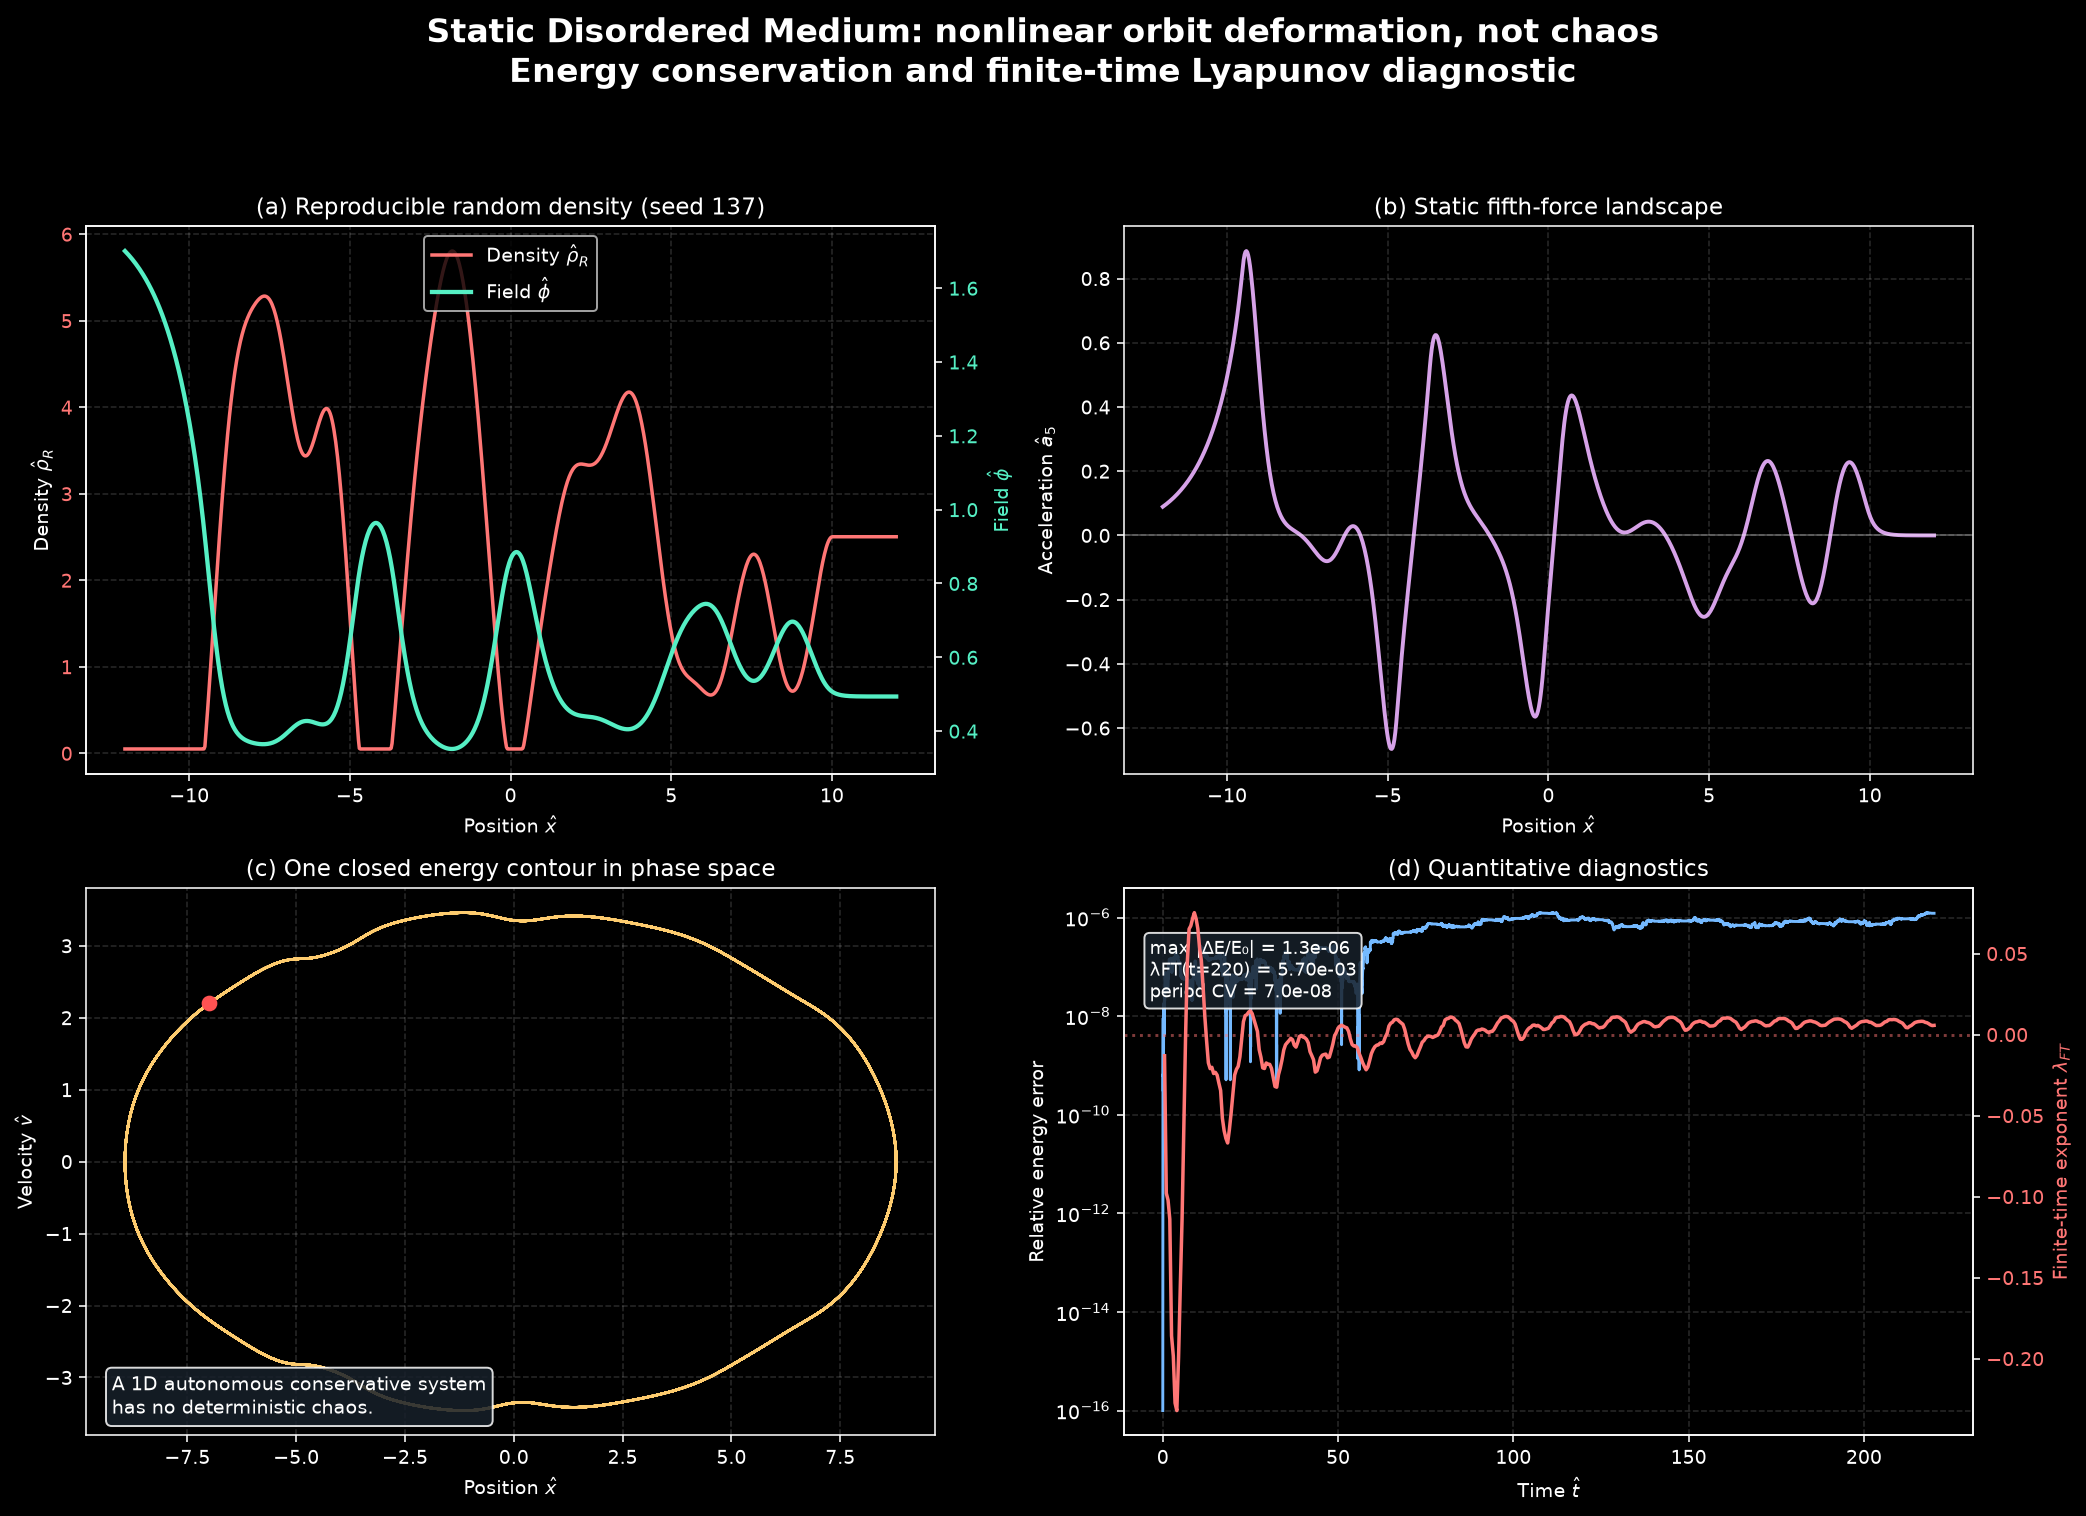
\includegraphics[width=0.94\textwidth]{chameleon_random_medium_results.png}
    \caption{정적 무작위 매질의 정량 진단. (a) 밀도와 장의 국소적 반응, (b) 위치에 따라 부호가 바뀌는 정적 제5의 힘, (c) 하나의 폐곡선을 이루는 위상 공간 에너지 등고선, (d) 상대 에너지 오차와 누적 유한시간 Lyapunov 지수. 복잡한 곡선 모양과 결정론적 카오스를 구분하였다.}
    \label{fig:random}
\end{figure}

\subsection{국소적 장 반응과 힘의 다중 구조}
고밀도 클럼프에서 $\hat\phi$는 작은 값으로 내려가고 저밀도 구간에서 커진다. 따라서 $-d\hat\phi/d\hat x$는 여러 양·음의 피크를 갖는다. 이 결과는 정적 밀도 요동이 복잡한 비선형 퍼텐셜을 만들 수 있음을 보이지만, ``무작위''라는 말은 공간 프로파일의 생성 방법을 가리킬 뿐 시간에 따른 확률적 힘이나 열적 브라운 운동을 뜻하지 않는다.

\subsection{왜 이 1차원 모형은 카오스가 아닌가}
본 입자 방정식은 시간에 무관한 1자유도 Hamiltonian
\begin{equation}
 H(\hat x,\hat v)=\frac{1}{2}\hat v^2+\frac{1}{2}\hat k\hat x^2+\hat\phi(\hat x)
\end{equation}
을 가지므로 적분 가능하다. 한 초기조건의 궤도는 $H=E$인 1차원 곡선을 따라 움직이며, 결정론적 카오스에 필요한 위상 공간의 접힘과 늘어남을 지속적으로 만들 수 없다. 이를 그림의 모양만으로 판단하지 않고 다음 지표로 확인하였다.

\begin{itemize}
 \item 최대 상대 에너지 드리프트는 약 $10^{-6}$ 수준으로 BVP 잔차와 보간 오차 범위에 머문다.
 \item 같은 방향의 $\hat x=0$ 통과로 정의한 귀환주기의 변동계수는 약 $10^{-7}$로, 궤도가 사실상 같은 주기를 반복한다.
 \item 변분방정식 $\dot{\delta x}=\delta v$, $\dot{\delta v}=a'(x)\delta x$을 함께 적분하고 0.5 시간마다 tangent vector를 재정규화하여 누적 유한시간 Lyapunov 지수 $\lambda_{\mathrm{FT}}(t)$를 계산하였다. 장시간 값은 0을 향해 감소하며 지속적인 양의 점근 지수를 보이지 않는다.
\end{itemize}

따라서 본 결과의 올바른 결론은 ``정적 무작위 퍼텐셜에 의한 비선형 궤도 변형''이다. 실제 카오스를 연구하려면 최소 2차원 산란계, 시간 의존 밀도장, 외부 주기 구동 중 하나를 도입하고 산란각 분포, Poincar\'e section, 장시간 Lyapunov spectrum을 계산해야 한다.

% ---------------------------------------------------------------------
% 7. 검출 가능성과 관측 제약
% ---------------------------------------------------------------------
\section{검출 가능성과 실제 물리 제약}

\subsection{원자 센서와 벌크 센서의 차이}
진공 챔버 안의 장 $\phi(r)$는 소스 질량, 잔류 기체, 챔버 벽과 경계조건이 결정한다. 시험 센서가 충분히 작다면 원자와 벌크 물질이 서로 다른 $\phi(r)$를 보는 것이 아니라 동일한 구배에 서로 다른 스칼라 전하로 반응한다.
\begin{equation}
 a_5=-Q_{\mathrm{test}}\frac{\beta}{M_{\mathrm{Pl}}}\nabla\phi,\qquad
 Q_{\mathrm{test}}\simeq\min\!\left(3\frac{\Delta R}{R},1\right).
\end{equation}
작고 비차폐된 원자는 $Q_{\mathrm{test}}\simeq1$일 수 있지만, 얇은 껍질을 가진 벌크 물질은 $Q_{\mathrm{test}}\ll1$이 되어 같은 구배에 대한 가속도 응답이 작다. 그림~\ref{fig:sensor}은 이 원리를 무차원 챔버 단면으로 나타낸 것이며 $Q_{\mathrm{bulk}}=0.03$은 설명용 값이지 특정 실험의 추정치가 아니다.

\begin{figure}[H]
 \centering
 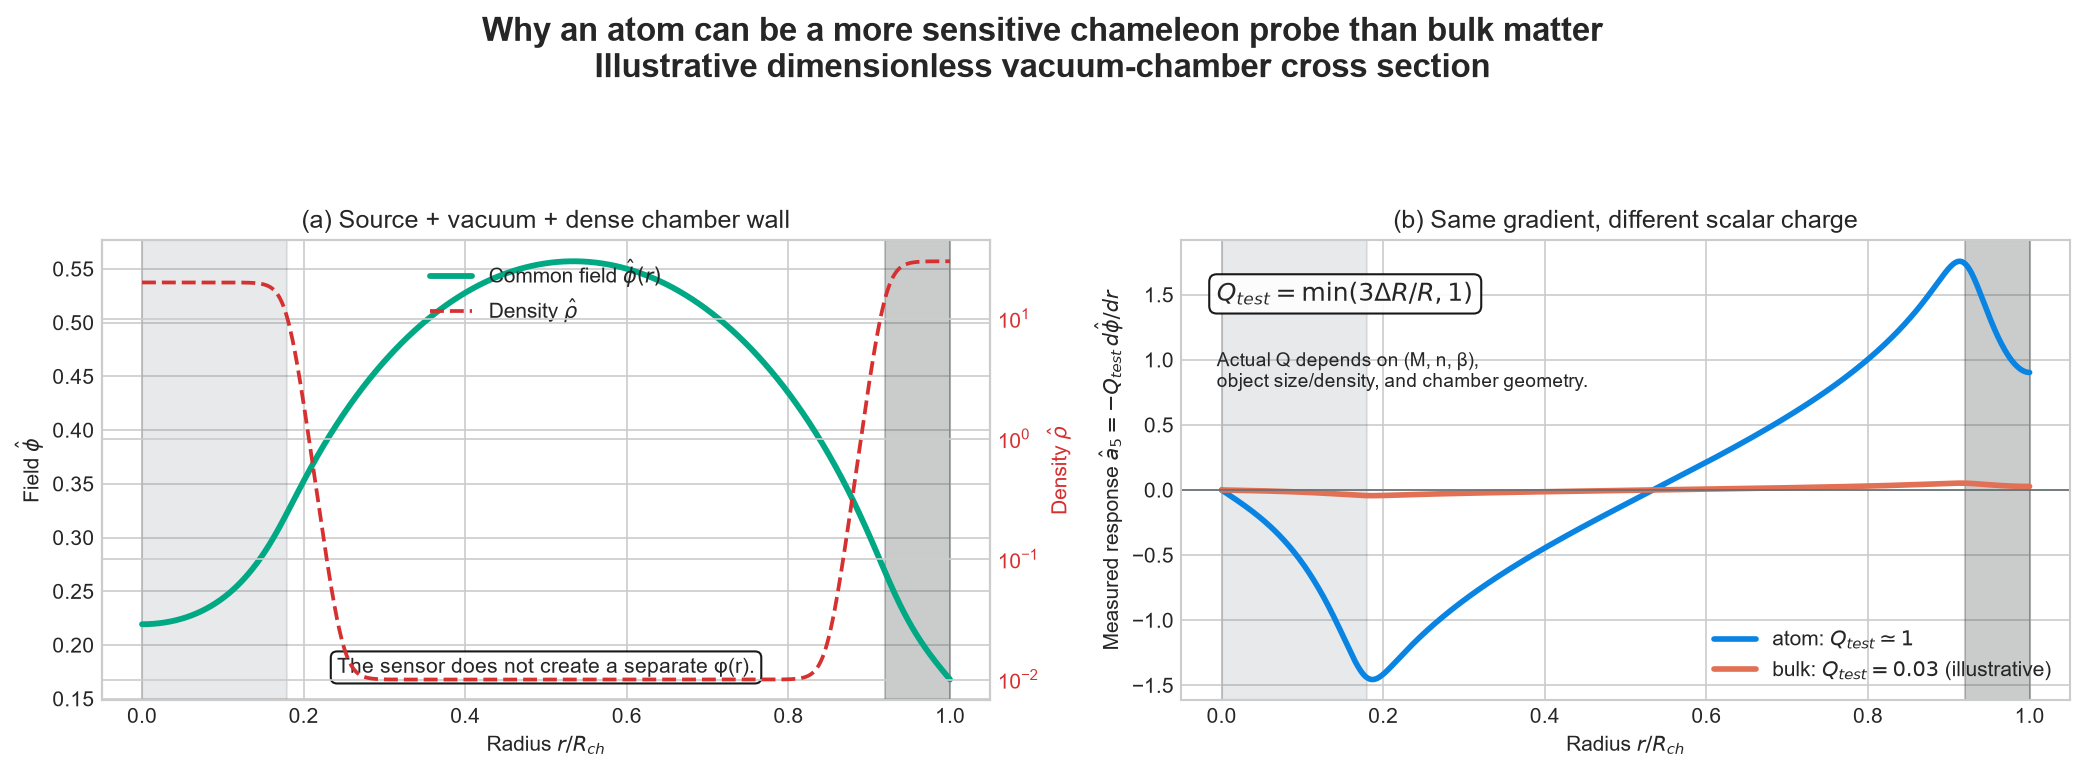
\includegraphics[width=0.96\textwidth]{sensor_detectability.png}
 \caption{진공 챔버의 공통 장 프로파일과 센서별 응답. 원자와 벌크 센서는 서로 다른 장을 보는 것이 아니라 서로 다른 $Q_{\mathrm{test}}$로 동일한 구배를 측정한다.}
 \label{fig:sensor}
\end{figure}

원자 간섭계는 초고진공 안에서 소스 질량의 위치를 바꾸고 원자 물질파의 위상 변화를 측정한다. Hamilton 등은 세슘 원자를 이용하여 스크리닝된 암흑에너지 모형을 제한하였고\cite{Hamilton2015}, Sabulsky 등은 루비듐 원자가 구형 소스 질량을 향해 받는 비정상 가속도에서 유의한 신호를 찾지 못해 추가 제약을 제시하였다\cite{Sabulsky2019}. 이는 ``실험실에서는 원리적으로 검출 불가능''하다는 뜻이 아니라, 차폐되지 않는 probe와 적절한 챔버 형상을 선택하면 검증 가능하다는 뜻이다.

\subsection{파라미터 제약과 천체물리학적 검출}
허용 여부는 $\beta$ 하나가 아니라 $(M,n,\beta)$와 소스·센서의 차폐, 챔버 크기, 환경 밀도의 함수이다. Burrage와 Sakstein의 종합 검토는 흔히 연구되는 모형들이 강하게 제한되지만 다른 퍼텐셜에는 남은 영역이 있음을 보여준다\cite{BurrageSakstein2018}. 2022년 부상형 힘 센서 실험은 암흑에너지 스케일에 맞춘 기본적인 inverse-power chameleon 모형에서 제5의 힘을 찾지 못하고 그 모형을 암흑에너지 후보로 강하게 배제하였다\cite{Yin2022}. 따라서 본 무차원 모형의 $\beta=1$을 ``관측적으로 허용된 값''이라고 결론내릴 수 없다.

천체물리학에서는 은하의 환경별 차폐 차이, 보이드 내부의 은하 운동과 렌즈 질량--동역학 질량 비교가 검출 통로가 된다. 실제 보이드 프로파일을 유한요소법으로 푼 연구에서는 선택한 허용 모형에서 $a_{\phi}/a_{\mathrm{Newt}}\sim10^{-6}$--$10^{-5}$이며, 보이드 깊이와 내부 밀도 구배가 핵심임을 보고하였다\cite{Tamosiunas2022}. 이는 본 프로젝트의 tanh 구배 실험과 개념적으로 연결되지만, 본 장난감 모형의 힘 크기를 그 수치와 직접 비교할 수는 없다.

% ---------------------------------------------------------------------
% 8. 결론 및 토의
% ---------------------------------------------------------------------
\section{결론 및 토의 (Discussion \& Conclusion)}

본 연구는 카멜레온 스크리닝 효과를 재현 가능한 무차원 고전 동역학계로 구현하고, 수치 방법과 물리적 해석을 독립적으로 검증하였다.

도출된 주요 결과는 다음과 같이 요약할 수 있다.
\begin{enumerate}
    \item \textbf{수치 방법의 투명성:} BVP collocation, RK45 오차 제어, 직접 RK4 구현, 경계조건과 허용오차를 명시하고 공개 저장소와 실행 절차를 제공하였다.
    \item \textbf{검증된 궤도 계산:} 조화진동자 해석해, 균일밀도 BVP 상수해, RK4 4차 수렴, RK4--RK45 일치, 에너지 보존을 통해 코드가 알려진 단순계와 보존법칙을 재현함을 확인하였다.
    \item \textbf{과도한 카오스 주장 정정:} 정적 1차원 무작위 매질은 복잡한 힘 구조를 만들지만 에너지와 귀환주기를 보존하며, 장시간 양의 Lyapunov 지수의 증거가 없다. 이는 수치적으로 만든 force landscape와 실제 카오스를 구분한 결과이다.
    \item \textbf{검출 가능성 연결:} 진공 챔버에서 원자와 벌크 센서의 차이를 $Q_{\mathrm{test}}$로 설명하고, 원자 간섭계와 우주 보이드가 실제 검증 통로임을 제시하였다.
\end{enumerate}

결론적으로 본 계산은 환경 밀도에 따른 장의 질량과 힘 구배 변화라는 카멜레온 메커니즘의 핵심을 일관되게 재현한다. 그러나 이것은 특정 물리 파라미터의 생존 가능성을 검증한 결과가 아니다. 다음 단계는 SI 또는 자연단위로 완전한 스케일을 지정하고, 실제 챔버 형상에서 소스와 센서의 thin-shell factor를 계산한 뒤, 공개된 $(M,n,\beta)$ exclusion contour와 동일한 좌표계에서 비교하는 것이다. 카오스 연구를 계속한다면 2차원 또는 시간 의존 모형으로 자유도를 확장해야 한다.

% =====================================================================
% 9. 참고문헌
% =====================================================================
\begin{thebibliography}{99}

\bibitem{Khoury2004prl}
J.~Khoury and A.~Weltman,
``Chameleon Fields: Awaiting Surprises for Tests of Gravity in Space,''
\textit{Physical Review Letters}, Vol.~93, p.~171104, 2004.
\href{https://doi.org/10.1103/PhysRevLett.93.171104}{https://doi.org/10.1103/PhysRevLett.93.171104}

\bibitem{Khoury2004prd}
J.~Khoury and A.~Weltman,
``Chameleon Cosmology,''
\textit{Physical Review D}, Vol.~69, p.~044026, 2004.
\href{https://doi.org/10.1103/PhysRevD.69.044026}{https://doi.org/10.1103/PhysRevD.69.044026}

\bibitem{RatraPeebles1988}
B.~Ratra and P.~J.~E.~Peebles,
``Cosmological consequences of a rolling homogeneous scalar field,''
\textit{Physical Review D}, Vol.~37, p.~3406, 1988.

\bibitem{Carroll1998}
S.~M.~Carroll,
``Quintessence and the rest of the world,''
\textit{Physical Review Letters}, Vol.~81, pp.~3067--3070, 1998.

\bibitem{BurrageSakstein2018}
C.~Burrage and J.~Sakstein,
``Tests of Chameleon Gravity,''
\textit{Living Reviews in Relativity}, Vol.~21, Art.~1, 2018.
\href{https://doi.org/10.1007/s41114-018-0011-x}{https://doi.org/10.1007/s41114-018-0011-x}

\bibitem{Hamilton2015}
P.~Hamilton, M.~Jaffe, P.~Haslinger, Q.~Simmons, H.~M\"uller, and J.~Khoury,
``Atom-interferometry constraints on dark energy,''
\textit{Science}, Vol.~349, pp.~849--851, 2015.
\href{https://doi.org/10.1126/science.aaa8883}{https://doi.org/10.1126/science.aaa8883}

\bibitem{Sabulsky2019}
D.~O.~Sabulsky, I.~Dutta, E.~A.~Hinds, B.~Elder, C.~Burrage, and E.~J.~Copeland,
``Experiment to Detect Dark Energy Forces Using Atom Interferometry,''
\textit{Physical Review Letters}, Vol.~123, p.~061102, 2019.
\href{https://doi.org/10.1103/PhysRevLett.123.061102}{https://doi.org/10.1103/PhysRevLett.123.061102}

\bibitem{Yin2022}
P.~Yin et al.,
``Experiments with levitated force sensor challenge theories of dark energy,''
\textit{Nature Physics}, Vol.~18, pp.~1181--1185, 2022.
\href{https://doi.org/10.1038/s41567-022-01706-9}{https://doi.org/10.1038/s41567-022-01706-9}

\bibitem{Tamosiunas2022}
A.~Tamosiunas, C.~Briddon, C.~Burrage, A.~Cutforth, A.~Moss, and T.~Vincent,
``Chameleon Screening in Cosmic Voids,''
\textit{Journal of Cosmology and Astroparticle Physics}, Vol.~2022, No.~11, p.~056, 2022.
\href{https://doi.org/10.1088/1475-7516/2022/11/056}{https://doi.org/10.1088/1475-7516/2022/11/056}

\end{thebibliography}

\end{document}
